\section*{Aspect Organisationnel}
\myparagraph{Diagramme}
\begin{center}
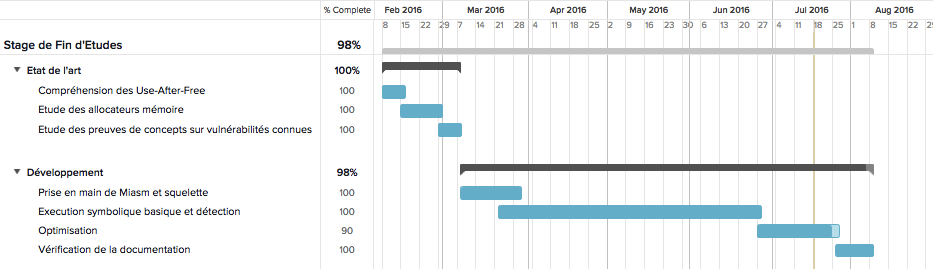
\includegraphics[scale=0.5]{gant.png}\newline
\end{center}

\myparagraph{Respect et critiques du découpage}
Le planning a été élaboré dans les grands traits lors de la première semaine de stage et a permis de bien structurer
le stage et les durées allouées à chacune des taches. L'ensemble du découpage a été respecté à la lettre. Les parties
concernant l'état de l'art été interrompues en cas d'échéance. En effet, les études étaient déjà assez avancées et le plus
important restait le developpement de l'outil en lui-même pour avoir un vrai cas pratique.

\myparagraph{Contrôle et réunion d'avancement}
L'avancée du projet a été suivi régulièrement avec un maximum de 2 semaines entre chaque point de contrôle. Durant ces réunions,
les points abordées étaient : les problèmatiques rencontrées, les futures étapes, les dates approximatives de fin de ces étapes.
\subparagraph{}
Le projet était également disponible sur un dépot de versionnement (git) sur l'infrastructure de l'ESEC. Des contrôles pouvaient donc être
fait même en dehors des séances de réunion. Des presentations étaient également effectuées toutes les deux semaines en début de stage, puis plus
espacées, afin de montrer le travail réalisé et poser des questions à l'équipe au complet.
